\documentclass[english,runningheads]{llncs}
\usepackage[T1]{fontenc}
\usepackage[utf8]{inputenc}
\usepackage{url}
\usepackage{graphicx}
\usepackage{babel}
\usepackage{multirow}
\usepackage[table,xcdraw]{xcolor}

\DeclareUnicodeCharacter{00D7}{$\times$}

\begin{document}
\title{Efficient static analysis of Marlowe contracts}

\author{Pablo {Lamela Seijas}\inst{1}\orcidID{0000-0002-1730-1219} \and
        David Smith\inst{1}\orcidID{0000-0003-1859-8007} \and
        Simon Thompson\inst{1,2}\orcidID{0000-0002-2350-301X}}

\authorrunning{P. Lamela Seijas, et al.}

\institute{IOHK, Hong Kong,
\email{pablo.lamela@iohk.io, david.smith@tweag.io, simon.thompson@iohk.io}  \and
School of Computing, University of Kent, UK,
\email{s.j.thompson@kent.ac.uk}}

\maketitle
\begin{abstract}
SMT solvers can verify properties automatically and efficiently, and they offer increasing
flexibility on the ways those properties can be described. However, the way in which
properties are described can affect the computational cost of verifying them considerably. In addition, it is hard to predict how changes on the way of describing a property
translate into changes to the computational costs.

In this paper, we discuss the lessons we have learned while implementing and optimising the static analysis functionality for Marlowe, a domain specific language for describing self-enforcing financial smart-contracts that can be deployed on a blockchain.
\end{abstract}
\section{Introduction\label{sec:Introduction}}

Thanks to static analysis, we can automatically check beforehand whether any
payments promised by a Marlowe contract can be fulfilled in every
possible execution of the contract. If a Marlowe contract has passed
the static analysis, we will have a very high assurance
that whenever the contract says we will be paid a certain amount of
money, any execution of the contract will indeed have enough money to
make such payment.

Marlowe's static analysis relies on SMT solvers, which are able to check whether a
set of constraints is satisfiable very efficiently. Thanks to state of the art
libraries like SBV \cite{erkok2019sbv}, we can describe those constraints in a
high-level language. In the case of SBV, we can directly write properties as
Haskell functions, with very few restrictions on how those functions are
implemented; SBV will automatically translate those functions into a language
that SMT solvers can understand (namely, SMTLib format \cite{barrett2010smt}).

Nevertheless, static analysis can become very computationally expensive if
implemented naïvely, because it needs to consider every possible value of the
property we want to check (in our case the main property we want to check
is whether a Marlowe contract will have enough money to make all the
payments described by the contract). Indeed, high-level abstractions
are often a tradeoff with efficiency.

For example, in the case of Marlowe, contracts are typically interactive
and must deal with inputs arriving from different users in different
orders, and sometimes not arriving at all. In addition, Marlowe allows
several inputs to be grouped in a single transaction, and different
decisions may be taken depending on the content of those inputs, or
in the combinations of contents of those inputs. All these alternatives
multiply the search space of static analysis and can easily compose
exponentially and thus make the whole approach unusable in practice
even for moderately sized contracts.

This paper contributes a number of approaches that can be used when
optimising static analysis, with examples extracted from a case-study where
we applied these approaches, an approach to ensure correctness
of the optimisations that combines the usage of property-based testing
and verification using automated theorem provers, and empirical data
that measures the effect of some of the optimisations on the implementation
of our case-study.

The case study presented is that of the optimisation of Marlowe's
static analysis. During this work, the techniques applied allowed
us to reduce the analysis time of an implementation that followed
the semantics closely and took a couple of minutes to analyse contracts
of a few kilobytes, to one where the same contract would take less
than a second, and where a four-person crowdfunding contract that
when fully expanded occupies about 19 megabytes, can be analysed in
around 10 minutes using Z3. In the original implementation, we were
not able to analyse the 19 megabyte contract because the analysis
ran out of memory after half an hour.

There are many things that can be done to improve the efficiency of
static analysis. We have classified them as lightweight and heavyweight. 

\paragraph*{Lightweight}

modifications are local and can be done without fundamentally changing
the implementation. We consider three main ideas:
\begin{itemize}
\item \textbf{Removing unnecessary parts from the analysis}. If they do not affect
the property that is being verified then we can just remove them from
the implementation and reduce its complexity.
\item \textbf{Avoiding high level abstractions}. High level abstractions aid reasoning
and avoid errors, but also introduce complexity that is not necessarily
needed.
\item \textbf{Reducing the search space by normalising parameters}. If there are several
ways of representing some inputs, and the different representations
have no impact on the analysis, we can remove all but one when
implementing static analysis.
\end{itemize}

\paragraph*{Heavyweight}

modifications are more fundamental approaches that require considerable
changes to the structure of the implementation. But these optimisations can also
translate in important reductions to execution time and memory usage, as
shown by the experiments we report in Section~\ref{sec:Measurements}.
We consider two main ideas:
\begin{itemize}
\item \textbf{Reducing the search space by using normalised execution paths relevant
to the property}. Instead of using the search space to model inputs, we
use it to model possible executions, and we ensure that we only
represent each possible group of equivalent executions once, i.e:
executions with the same normal form (or equivalence partitioning).
\item \textbf{Minimizing the representation of inputs and outputs}. We can benefit
from encoding inputs and outputs as concisely as possible, and discarding
information that we can infer in other ways.
\end{itemize}
In the following sections, we introduce the semantics of Marlowe as
a case study (Section~\ref{sec:Marlowe-intro}), we cover a
general approach to static analysis (Section~\ref{sec:Making-Marlowe-symbolic}),
we then explore both lightweight (Section~\ref{subsec:Lightweight-modifications})
and heavyweight (Section~\ref{subsec:Heavyweight-modifications})
optimisation techniques in more detail, and we illustrate them with
examples of how they apply to Marlowe static analysis. In Section~\ref{sec:Testing},
we briefly discuss some ways in which property based testing can be
used to address potential problems that may arise from the implementation
of the heavyweight optimisations described in the previous section.
In Section~\ref{sec:Measurements}, we present empirical results that
show the effects of heavyweight optimisations on the execution time
and memory usage of Marlowe's static analysis.

\section{Marlowe and how its design helps static analysis and correctness\label{sec:Marlowe-intro} }

Firstly, we will briefly introduce the semantics of Marlowe, the guarantees
that are offered implicitly by the semantics, and how the design choices
facilitate static analysis and make it decidable. A more detailed
explanation of Marlowe can be found in \cite{marlowe}.

\subsection{Structure of Marlowe contracts\label{subsec:Structure-of-Marlowe} }

The Marlowe language is realised as a set of mutually recursive Haskell
data types. Marlowe contracts regulate interactions between a finite number
of participants, determined before the contract is deployed.

Marlowe contracts are able to receive payments, store money and tokens,
ask for input from the participants, and redistribute stored money
and tokens back among participants. The decision about which and when of
these actions are carried out is determined by the contract on the basis
of the information that is available at each point in time. Participants
may correspond to either individual public keys or to tokens (\texttt{Role}s).
In turn, \texttt{Role}s may be controlled by separate independent contracts.

The main data type in Marlowe is called \texttt{Contract}, and it represents
the logic and actions that the contract allows or enforces. The outmost
constructs of the \texttt{Contract} represent the actions that will be enforced
first and, as those constructs become enforced, the \texttt{Contract} will
evolve into one of its continuations (sub-contracts), and the process
will continue until only the construct \texttt{Close} remains.

There are 5 constructs of type \texttt{Contract}:
\begin{itemize}
\item \texttt{Close} -- signals the end of the life of a contract. Once
it is reached, all the money and tokens stored in the accounts of
the contract will be refunded to the owner of each of the respective
accounts.
\item \texttt{If} -- immediately decides how the contract must continue
from between two possibilities and depending on a given Boolean condition
that we call an \texttt{Observation}. The value of an \texttt{Observation}
can depend on previous choices made by participants, on amounts of money
and tokens stored in the contract, or other factors.
\item \texttt{Let} -- immediately stores a \texttt{Value} for later use.
Expressions of type \texttt{Value} in Marlowe are evaluated to integer
values and they depend on information available to the contract at the
time of evaluation. For example, a \texttt{Let} construct can be used to
store the amount of money available in a particular account at a given point
in time, for use at a later stage of the contract execution.
\item \texttt{When} -- waits for an external input. The \texttt{When} construct
also specifies a timeout slot\footnote{Slots are blockchain's proxy for time,
they are added to the blockchain periodically.}: after this slot has been reached, the
\texttt{When} construct expires, and no longer accepts any input.
There are three kinds of input:
\begin{itemize}
\item \texttt{Deposit} -- Waits for a participant to deposit an amount
of money or tokens (specified as a \texttt{Value}) in an account of the contract.
\item \texttt{Choice} -- Waits for a participant to make a choice. A choice
is represented as an integer number from a set specified by the contract.
\item \texttt{Notify} -- Waits for an \texttt{Observation} to be true.
Because contracts are reactive (they cannot initiate transactions),
it is necessary for an external actor to \texttt{Notify} the contract
that the \texttt{Observation} has become true. However, this notification
does not have to be carried out by a participant, anybody can do it.
\end{itemize}
\item \texttt{Pay} -- immediately makes a payment between accounts of the
contract, or from an account of the contract to a given participant.
The amount transferred is specified as a \texttt{Value}.
\end{itemize}

\subsection{Semantics\label{subsec:Marlowe-Semantics}}

As we mentioned in the previous section, Marlowe
contracts are passive: their code is executed as part of the validation of
transactions that are submitted to the blockchain. These transactions
need to be submitted by participants or their representatives (e.g.
user wallets) and their validation is carried out atomically and
deterministically.

Each transaction may include a list of inputs, a set of signatures,
a slot interval\footnote{We use a slot interval because it is very difficult to
know in practice in which slot the transaction is going to be included,
and we need transactions to be deterministic, so we cannot use individual
slot numbers.}, a set of input UTxOs (incoming money and tokens), and a
set of outputs (outgoing money and tokens). For
a transaction to be valid in Marlowe, the transaction must have the
same effect for every slot within that slot range (be deterministic).
For example, if a transaction has a minimum slot number which is before
a timeout, and a maximum slot which after a timeout then the transaction
will fail with the error \texttt{AmbiguousSlotInterval}, since it would
not be deterministic.

A key aspect of the Marlowe semantics is that it checks that a particular
transaction is valid given the current state and contract. Because
transactions are deterministic, there should be no reason why someone
accidentally sends a transaction that is invalid for a given \texttt{State}
and \texttt{Contract}, since it will only result in a cost to that participant.
However, it is still possible that, due to a race condition, a participant will send a
transaction that no longer applies to a running \texttt{Contract} and
\texttt{State}, but such a transaction would simply be ignored by the
blockchain.

The type signature of the transaction validation function is:

\begin{verbatim}
computeTransaction :: TransactionInput -> State -> Contract
                   -> TransactionOutput 
\end{verbatim}

This function can be factored into four main functions:
\begin{itemize}
\item \texttt{reduceContractStep} - this function executes the topmost
construct that does not require an input to be executed (i.e: anything
but a \texttt{When} that has not expired or a \texttt{Close} when
accounts are empty). It only simplifies the \texttt{When} construct
if it has expired (i.e. the timeout specified in the \texttt{When}
is less than or equal to the minimum slot number). In the case of
the \texttt{Close} contract, it only refunds one of the accounts at
each invocation. 
\item \texttt{reduceContractUntilQuiescent} - this function calls \texttt{reduceContractStep}
repeatedly until it has no further effect,
\item \texttt{applyInput} - this function processes one single input.
The topmost construct must be a \texttt{When} that
is expecting that particular input and has not expired. 
\item \texttt{applyAllInputs} - this function processes a list of inputs.
It calls \texttt{applyInput} for each of the inputs in the list, and
calls \texttt{reduceContractUntilQuiescent} before and after every
call to \texttt{applyInput}.
\end{itemize}
The \texttt{State} stores information about the amount of money and
tokens in the contract at a given time, together with the choices
made, \texttt{Let} bindings made, and a lower bound for the current
slot:

\begin{verbatim}
data State = State { accounts    :: Map AccountId Money
                   , choices     :: Map ChoiceId ChosenNum
                   , boundValues :: Map ValueId Integer
                   , minSlot     :: Slot }
\end{verbatim}

\subsection{Extra considerations\label{subsec:Extra-considerations}}

Many of the design decisions behind Marlowe have been made with the
aim of preventing potential errors. For example:
\begin{itemize}
\item \textbf{Classification of money and tokens into accounts} separates concerns.
A Marlowe contract will never spend more money or tokens than there are in an
account, even if there is more available in the contract. But when
required to pay more than is in an account, it will pay as much as
is available in the account, in order to remain as close as possible
to the original intention of the contract.
\item \textbf{Account identifiers include an account owner}. An account owner
is a participant that will get the money or tokens remaining in an account
when a contract terminates. At the same time, the only construct that
can pause the execution of a contract is the \texttt{When} construct,
which has a timeout, this ensures that all contracts eventually expire
and terminate. Together, these properties ensure that no money or tokens
are locked in the contract forever.
\item \textbf{No negative deposits or payments}. Marlowe treats negative
amounts in deposits and payments as zero. However, at the same time,
if there happens to be a request for deposit with a negative amount,
it continues gracefully: it will still wait for a null deposit to
be made, and it will continue as if everything is correct; this way,
the expected execution of the contract is disturbed as little as possible.
\item \textbf{Upper limit in the number of inputs} that a Marlowe contract
can accept throughout its lifetime. This limit is implied by the maximum
number of nested \texttt{When} constructs in the contract, since only one input
per \texttt{When} can be accepted. At the same time, transactions that have
no effect on the contract are considered invalid, thus there is also
a limit in the maximum number of transactions a contract can accept
throughout its life. This bound prevents DoS attacks, and it makes static analysis
easier. We discuss this in more detail in Section~\ref{sec:Making-Marlowe-symbolic}.
\end{itemize}

\section{Making Marlowe semantics symbolic\label{sec:Making-Marlowe-symbolic}}

In this section, we briefly present and reflect on a technique that
can be used to convert a concrete implementation of a Haskell function
into a symbolic one by using the SBV library \cite{erkok2019sbv}, and to use this symbolic
implementation for static analysis. In particular, we explore this
technique in the context of the Marlowe semantics.

This approach corresponds to our first attempt at implementing static
analysis for Marlowe contracts, and it is a systematic approach that
can be carried out with very few assumptions. 

\subsection{Overview}

The SBV library supports implementing Haskell functions in a way that
the same implementation can be used:
\begin{itemize}
\item With concrete parameters, as a normal Haskell function
\item With symbolic variables, so that properties can be checked for satisfiability
using an SMT solver
\item As part of QuickCheck properties, for random testing.
\end{itemize}
Parameters that can be used symbolically are wrapped in a monad called
\texttt{SBV}. Functions that depend on symbolic parameters also return
values wrapped in the \texttt{SBV} monad.

The idea is therefore to convert our implementation to use values
wrapped in the \texttt{SBV} monad, by replacing all operations on
those values with symbolic functions. In order to simplify this work,
\texttt{SBV} provides symbolic versions for many of the most common
built-in functions that are either overloaded or have similar names.

Our semantics transaction processing function would thus become:

\begin{verbatim}
computeTransaction :: SBV TransactionInput -> SBV State
                   -> SBV Contract
                   -> SBV TransactionOutput
\end{verbatim}

We can then define a function that takes a list of transactions instead,
and we would just need to write a property that says that the result
of executing the list of transactions for a given contract does not
have any warnings (the property we are trying to verify). Then we
can pass the property to SBV and it will tell us which transaction
lists break the property.

Unfortunately, there are a couple of issues with this approach that
we review in Section~\ref{subsec:considerations}.

\subsection{Additional considerations\label{subsec:considerations}}

SBV does not currently support complex custom data types. At the time
of writing, SBV has some support for 0-ary data types, but not for
data types with parameters.
It does provide symbolic versions of the \texttt{Either} type and the \texttt{Tuple} type.
Thus, it is possible to have an isomorphism between custom data types and
nested \texttt{Either} and \texttt{Tuple} type-synonyms. Our original
implementation automatically generates conversion functions between these
by using Template Haskell \cite{sheard2002template}. By using this technique the symbolic
implementation can remain similar to the concrete one.

For example, the following data structure:

\begin{verbatim}
data Input = IDeposit AccountId Party Money
           | IChoice ChoiceId ChosenNum
           | INotify
\end{verbatim}

Would be translated to the following type synonym:

\begin{verbatim}
type SInput = SBV (Either (AccountId, Party, Money)
                          (Either (ChoiceId, ChosenNum)
                                  ()))
\end{verbatim}

But this approach cannot address recursive datatypes, let alone mutually
recursive datatypes. And the \texttt{Contract} type is mutually recursive.

Even if we could represent mutually recursive datatypes, it would
not be feasible to directly translate the semantics, because a more
general limitation of SMT solvers is that they cannot, in general,
deal with arbitrarily sized computations. In other words, if termination
of a symbolic function is not bounded, or is only bounded by a symbolic
parameter, SMT solvers will often fail to terminate when trying to validate
a property, since doing so often requires a proof by induction. We
discuss how to address this problem in Section~\ref{subsec:Adapting-the-semantics}.

\subsection{Adapting the semantics\label{subsec:Adapting-the-semantics}}

In order to guarantee termination of the SMT validation, we need a
concrete bound for the property that we want to validate.

Related work often addresses this problem by manually establishing
a bound on the amount of computation, e.g: limiting the number of
computation steps analysed, the number of times loops are unrolled
\cite{clarke2004tool,gulwani2008program,jackson2000finding}.

In the case of Marlowe, we have natural bounds that we can use because,
given a concrete contract, we can easily infer:
\begin{itemize}
\item The maximum number of inputs that can have an effect on the contract
\item The maximum number of transactions that can have an effect on the
contract
\item All of the account, choice, and \texttt{Let} identifiers that will
be used in the contract
\item The number of participants that will participate in the contract
\end{itemize}
From this data, we can also deduce an upper bound for:
\begin{itemize}
\item The number of times that
\texttt{computeTransaction}, \texttt{reduceContractStep}, and \texttt{applyInput} may
be called.
\item The number of accounts that the contract will use, and an
the number of elements there may be in each of the associative maps
that comprise the \texttt{State} of the contract at any given point
of the execution.
\end{itemize}
If we keep the \texttt{Contract} parameter concrete,
we can use it to bound the execution, because every call to \texttt{reduceContractStep}
will either make no progress or remove one of the constructs, with
the exception of \texttt{Close}. But for any particular \texttt{Contract},
we know we only need to call \texttt{reduceContractStep} at most as many times as
the maximum number of accounts there can possibly be, since, every time we call
it, it will refund one of the accounts.

Thus, the symbolic transaction processing function becomes:

\begin{verbatim}
computeTransaction :: SBV TransactionInput -> SBV State
                   -> Contract
                   -> SBV TransactionOutput
\end{verbatim}

There is one more problem: the output \texttt{Contract} returned
by the function, which is wrapped inside the \texttt{TransactionOutput},
is symbolic, since it depends on the current \texttt{TransactionInput}
and \texttt{State}, which are both symbolic.

We get around this problem by using a continuation style. Instead
of returning the \texttt{TransactionOutput} directly, we take a continuation
function that takes the concrete \texttt{Contract} and the symbolic version
of \texttt{TransactionOutput} without the \texttt{Contract}.

Thus, the symbolic transaction processing function will look something
like:

\begin{verbatim}
computeTransaction :: SymVal a => SBV TransactionInput
                   -> SBV State -> Contract
                   -> (SBV TransactionOutput ->
                       Contract -> SBV a)
                   -> SBV a
\end{verbatim}

In practice, we also include some extra information about bounds,
and we make some other parts of \texttt{TransactionOutput} concrete,
in addition to the \texttt{Contract}.

\section{Making static analysis more efficient\label{sec:Making-static-analysis-efficient}}

In this section, we explain, in more detail, the techniques that we mentioned
in the introduction, and we illustrate those techniques with
examples from the static analysis implementation of Marlowe.

\subsection{Lightweight modifications\label{subsec:Lightweight-modifications}}

Some of the modifications that we can apply to a static analysis implementation
are localised, and they do not fundamentally affect the overall structure
of the implementation. This means that the implementation can remain close
to the original semantics and model that we are
trying to analyze, as well as making changes less likely to introduce
errors than a more serious restructuring.

\subsubsection{Removing unnecessary parts from the analysis.}

This is probably the most straightforward optimization to implement.
When we use the same or similar code for both the analysis and the
implementation, we may end up including code that is not relevant
to the analysis.

In the case of Marlowe, this was the case of the \texttt{Close} construct.
The \texttt{Close} construct refunds all the money and tokens remaining
in the accounts. At the time of analysis, we do not know how much
is available in each account, because it may depend on the value of
a choice made by the user in runtime. For that reason, the generated
constraints must include comparisons for every account. This makes
the implementation of the \texttt{Close} construct very expensive
to execute symbolically.

As it turns out, we do not need to implement the semantics of the
\texttt{Close} construct at all, because it is impossible for the
\texttt{Close} construct to produce a failed payment
(we have also proven this\footnote{\url{https://github.com/input-output-hk/marlowe/blob/master/isabelle/CloseSafe.thy} (last visited on 04/04/2020)} using Isabelle \cite{nipkow2002isabelle}): it only pays whatever there is available.
So we can safely remove it from the analysis.

\subsubsection{Avoiding high level abstractions.}

High level libraries like SBV, and even standards like SMTLib, support
the use and construction of high level abstractions,
e.g: custom data-types, list, sets\dots{} Unfortunately, even though
high level abstractions make reasoning about code easier, they often
prevent certain optimisations, since they abstract out aspects of
the implementation that in our particular case may be concrete.

For example, in the case of Marlowe's static analysis, we initially
implemented a \emph{symbolic} associative map primitive with the only limitation
that it needed a concrete bound in the number of elements. This is
straightforward to realise using the symbolic implementation of list
and tuple, both provided by SBV. However, this can be very costly:
searching a list symbolically requires constraints that check
the key of every element in the list up to the maximum capacity of
the associative map, because it is not known at the time of symbolic
execution how many elements the list has.

However, in Marlowe we know the values of all the keys that we are
going to use in maps, because the contract is concrete, and only \texttt{Account},
\texttt{Choice}, and \texttt{Let} identifiers that are mentioned in
the contract will ever make it into the \texttt{State}. So we do not
need keys of the associative map to be symbolic, we can use a concrete
associative map with symbolic values.

Nevertheless, using a partially concrete map prevents us from using
it as the result of a function that takes symbolic parameters, so
we will need to use a continuation style insead. An alternative is
to assign numbers to each possible key, and store them in a symbolic
list, this will at least prevent the search from having to compare
a lookup with every key, since we will know in which position of the
list each value is stored. 

\subsubsection{Reducing the search space by normalising parameters.
\label{subsec:Reducing-search-space-by-normalising-parameters}}

The higher the number of degrees of freedom of the input, the larger
the search space, and the higher the load we are putting on the SMT
solver. In many cases, we do not need to explore the whole search
space to check satisfiability of a property. In particular, we may
be able to prove that some sets of inputs are equivalent in terms
of the property whose satisfiability we want to test.

For example, in the case of Marlowe's static analysis,
Marlowe allows several inputs to be combined into a single transaction.
This functionality is important because each transaction requires
the issuer to pay fees, so combining several inputs in a single transaction
can translate into important savings. On the other hand, it also means
that static analysis must consider many more possibilities, since
the number of ways of partitioning inputs in transactions grows exponentially
in the number of inputs.

However, we can devise a normal form for input traces, in which there
is a maximum of one input per transaction. We only need to make sure
that, for every trace, if it produces a warning, there exists a trace
with only one input per transaction that also produces a warning.
Using the automated proof assistant Isabelle \cite{nipkow2002isabelle},
we have shown that, indeed, splitting transactions into transactions
with single inputs and the same slot interval as the original transactions
does not modify the effect of those transactions on a contract\footnote{\url{https://github.com/input-output-hk/marlowe/blob/master/isabelle/SingleInputTransactions.thy}
(last visited on 29/04/2020)}.

This optimization reduces the search space considerably, but transactions
may still have no inputs, so there are still many ways of distributing
the inputs in transactiongs. We explain how we reduced
the search space even further in Section~\ref{subsec:Heavyweight-modifications}. 

\subsection{Heavyweight modifications. \label{subsec:Heavyweight-modifications}}

When optimising, if our solution is a local minimum, small changes
to the parameters will not grant any improvement to the result.
For that reason, in this section, we explore ways of optimizing that
may imply considerable rewriting of our properties, constraints, and
static analysis implementation in general.


\subsubsection{Reducing the search space by using normalised execution paths relevant
to the property. \label{subsec:Reducing-search-space-by-using-normalised-execution-paths-relevant-to-the-property}}

One approach we can use that helps improve static analysis efficiency
is to focus on the property we want to test instead of trying to make
it as close as possible to the full implementation
of the system. We do not even need to think about the representation
of a counterexample (we will discuss that in the next section), but
only in what are the conditions for the property to be false.

Unfortunately, having static analysis be very different from implementation
makes the approach much more error prone, and in making an argument
for the trustworthiness of the analysis there are many more assumptions
that need to be made and reasoned about. In Section~\ref{sec:Testing},
we explore ways of mitigating this problem.

For example, the main property we want to check is whether there is
any possible execution that produces a failed payment. Thus, we look
at executions instead of looking at inputs. The most complicated construct
in terms of executions is the \texttt{When} construct, since it allows
for two transactions that are separate in time to have different effects
depending on when they are issued, all other constructs will get resolved
instantly in one way or another. But, without loss of generality,
we can structure them as Figure~\ref{fig:Distribution-of-transactions}
shows: we can conceptually break the contract tree into subtrees,
where each subtree has a \texttt{When} construct as its root, with
the exception of the subtree at the root of the original tree.

\begin{figure}
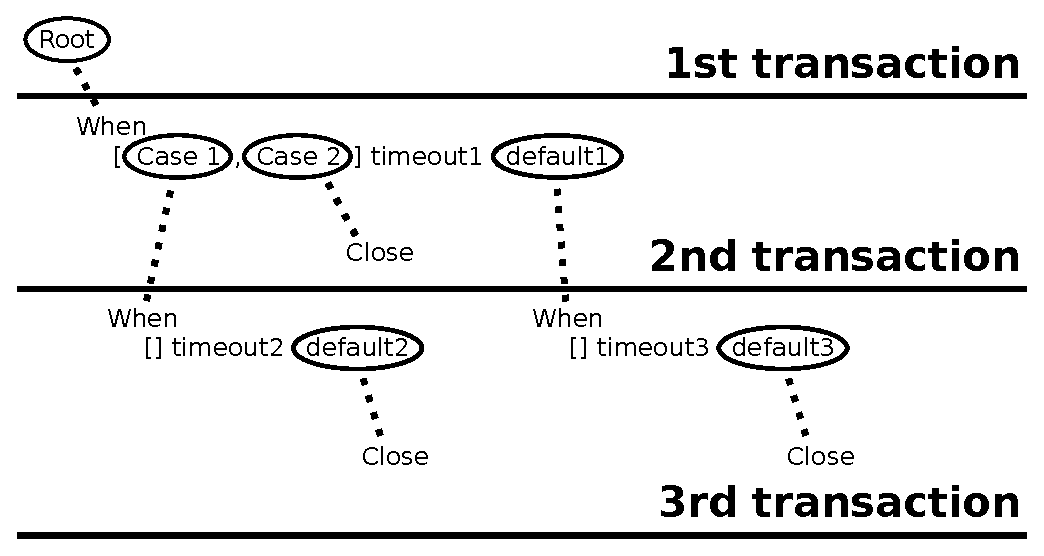
\includegraphics[width=1\textwidth]{figures/transactions}

\caption{Distribution of transactions with respect to a contract\label{fig:Distribution-of-transactions}}

\end{figure}

Each level of subtrees will correspond to a transaction, i.e: the
root subtree will correspond to the first transaction, the set of
subtrees that are children of the first subtree (in the original tree)
will correspond to the second transaction, and so on. There may be
some paths which do not require as many transactions/subtrees as other
paths, because they traverse fewer \texttt{When} constructs before
finding a \texttt{Close} construct.

We can assign one transaction to each segment of execution
before starting at a \texttt{When} or the root of the tree,
because if the maximum slot number of the
transaction is lower than the slot number in the timeout and the
transaction has no inputs, then the execution will stop before the
\texttt{When}, so we need to account for that possibility. In other
words, if two parts of the execution path may have different slot
numbers when we go through them, we need to consider them as separate
transactions, because they may have payments that depend on those values.

On the other hand, this segmentation is not general enough, because there is
an edge case. A transaction may execute past a \texttt{When} if the minimum
slot number in the transaction is greater or equal than the timeout of the
\texttt{When}. If the transaction expires the \texttt{When} we can no longer
separate the execution before the \texttt{When} and after the \texttt{When}
into two different transactions, because we know that the timeout branch of the
\texttt{When} will be executed as part of the first transaction, and thus
it will use the slot interval of the first
transaction (same used for the first segment).

This is not only true for the timeout branch, if we include
an input that is allowed by the \texttt{When} into the first transaction,
then the first transaction will continue into the corresponding \texttt{When}
branch, and we will not use a second transaction.

We cannot just constrain the maximum slot number of the first transaction
to be less than the timeout in the \texttt{When} because, if we do
that, then we will miss executions where one transaction expires several
\texttt{When} in a row, or where it expires one \texttt{When} and provides
the right input for later \texttt{When}. And we cannot just not constrain
the maximum slot number of the first transaction because then we will
not know to which segments each transaction applies.

We get around this problem by allowing the slot numbers of the first
and second transactions to be equal. If this happens, we will find
out that one of the transactions will be marked as \texttt{UselessTransaction}
by the semantics when we look at the counterexample. So we just need
to filter out all transactions that produce \texttt{UselessTransaction}
warnings in the final result.

Note however that, in Section~\ref{subsec:Reducing-search-space-by-normalising-parameters},
we already reduced the number of inputs per transaction to a maximum
of one, and the number of transactions to the maximum number of nested
\texttt{When}s plus one. But now we have also assigned each of the
transactions to a part of the contract, so we do not need a symbolic
list of transactions, we can have a finite concrete list of symbolic
transactions and we know in advance which of the transactions we are
working on at each moment during the symbolic execution.

One detail that we realised during testing is that, even though
the diagram above shows that a \texttt{When} belongs to the new transaction,
because the \texttt{When} will not be consumed by the previous transaction,
\texttt{Observation}s in the \texttt{Notify} cases will correspond to the
information there was in the \texttt{State} before the \texttt{When}
was executed, with the exception of the slot interval, which will still be
considered to be that of the transaction that triggers the \texttt{When} (the
new transaction). The same is true for \texttt{Value}s in the \texttt{Deposit}
cases, since the amount to deposit must be calculated without considering the
effects of the deposit itself, we need to refer to the \texttt{State} before
the deposit was made.

\subsubsection{Minimizing the representation of inputs and outputs.}

When we initially implemented the efficient version of static analysis
for Marlowe, we did not pay any attention to the inputs and outputs.
The first version would simply take a concrete \texttt{Contract}
as input, and it would return a symbolic Boolean that determined whether
the \texttt{Contract} was valid or not. However, if a \texttt{Contract}
turns out to be invalid, we will also want to know why, so we later modified
the property to give a counterexample that illustrated what went wrong.
The original implementation still used some intermediate symbolic
variables, but they were anonymous, and they were created during the
exploration of the contract.

A simple way of obtaining a counterexample is to modify the output
of the function to return the offending trace using the symbolic \texttt{Maybe}
type. Surprisingly, this small change increases the amount of time
required by the symbolic analysis severalfold.

The solution to this increase in execution time was to pass as input, to
the static analysis implementation, a fixed list, with each element corresponding
to a transaction and consisting of a tuple with four symbolic integers:
\begin{enumerate}
\item An integer representing the minimum slot
\item An integer representing the maximum slot
\item An integer representing the \texttt{When} case whose input is being
included in the transaction, where zero represents the timeout branch
(and there being no inputs to the transaction).
\item An integer representing the amount of money or tokens (if the input
is a \texttt{Deposit}), or the number chosen (if the input is a \texttt{Choice})
\end{enumerate}
If we need fewer transactions, we will just add dummy transactions with all four numbers
set to $-1$ at the end of the list.

In order to translate this sequence of numbers into a proper list
of transactions that is human readable and we can use to report the
counter example, we need to iterate through the list and see the evolution
of the contract with each transaction, using the concrete semantics.
This way, we can gather the rest of necessary information, such as
whether the transaction input is a \texttt{Deposit}. We can also see
which of the transactions do not have an effect, i.e: they produce
\texttt{UselessTransaction} as we mentioned in Section~\ref{subsec:Reducing-search-space-by-using-normalised-execution-paths-relevant-to-the-property}.

We use this separation of concerns between the static analysis and
the concrete semantics to our advantage, as an opportunity for applying
property based testing, as we explain in Section~\ref{subsec:Testing-for-consistency}.

\section{Testing for consistency and equivalence\label{sec:Testing}}

Errors often occur when optimising or translating. If the static analysis
implementation is close to the actual implementation, it is much less
likely that a mistake will be made when writing it. On the other hand,
if we have to craft a static analysis implementation that is equivalent
(in some sense) to the original, but is written in a very different
way, it is more likely that we will make assumptions which do not
hold.

In order to avoid these problems, we combine the use of automated proof
assistants to verify our assumptions and the use of property based testing to
test for consistency and equivalence (as we describe in
Section~\ref{subsec:Testing-for-consistency}).

\subsection{Testing for consistency\label{subsec:Testing-for-consistency} }

If our static analysis does not replicate all the functionality of
the semantics, we can use potential discrepancies as an opportunity
for testing, as shown in Figure~\ref{fig:Property-based-testing-for-consistency}.
We generate random contracts and we apply the static analysis to them
in order to try to find a counterexample that produces warnings. If
we cannot find any counterexamples then the test passes, but if we
find one, we can test it on the semantics and see whether the counterexample
indeed produces warnings in the semantics too, if it does not we have
found a problem in either the static analysis or the semantics.

A limitation of this approach is that it only tests for false positives,
and it does not prevent false negatives, but those can be covered by testing
for equivalence (see Section~\ref{subsec:Testing-for-equivalence}).

In addition, we can add assertions to the process. In the case of
Marlowe, if the counterexample causes errors during the execution or is
formed incorrectly, it would also mean that there is a problem with
the static analysis. For example, it may be that the counterexample
refers to a \texttt{Case} of a \texttt{When} that does not exist,
or that it has invalid or ambiguous intervals. If it has \texttt{UselessTransactions}
is ok, because we are doing that on purpose, as we mentioned in Section~\ref{subsec:Reducing-search-space-by-using-normalised-execution-paths-relevant-to-the-property}.

\begin{figure}
\begin{centering}
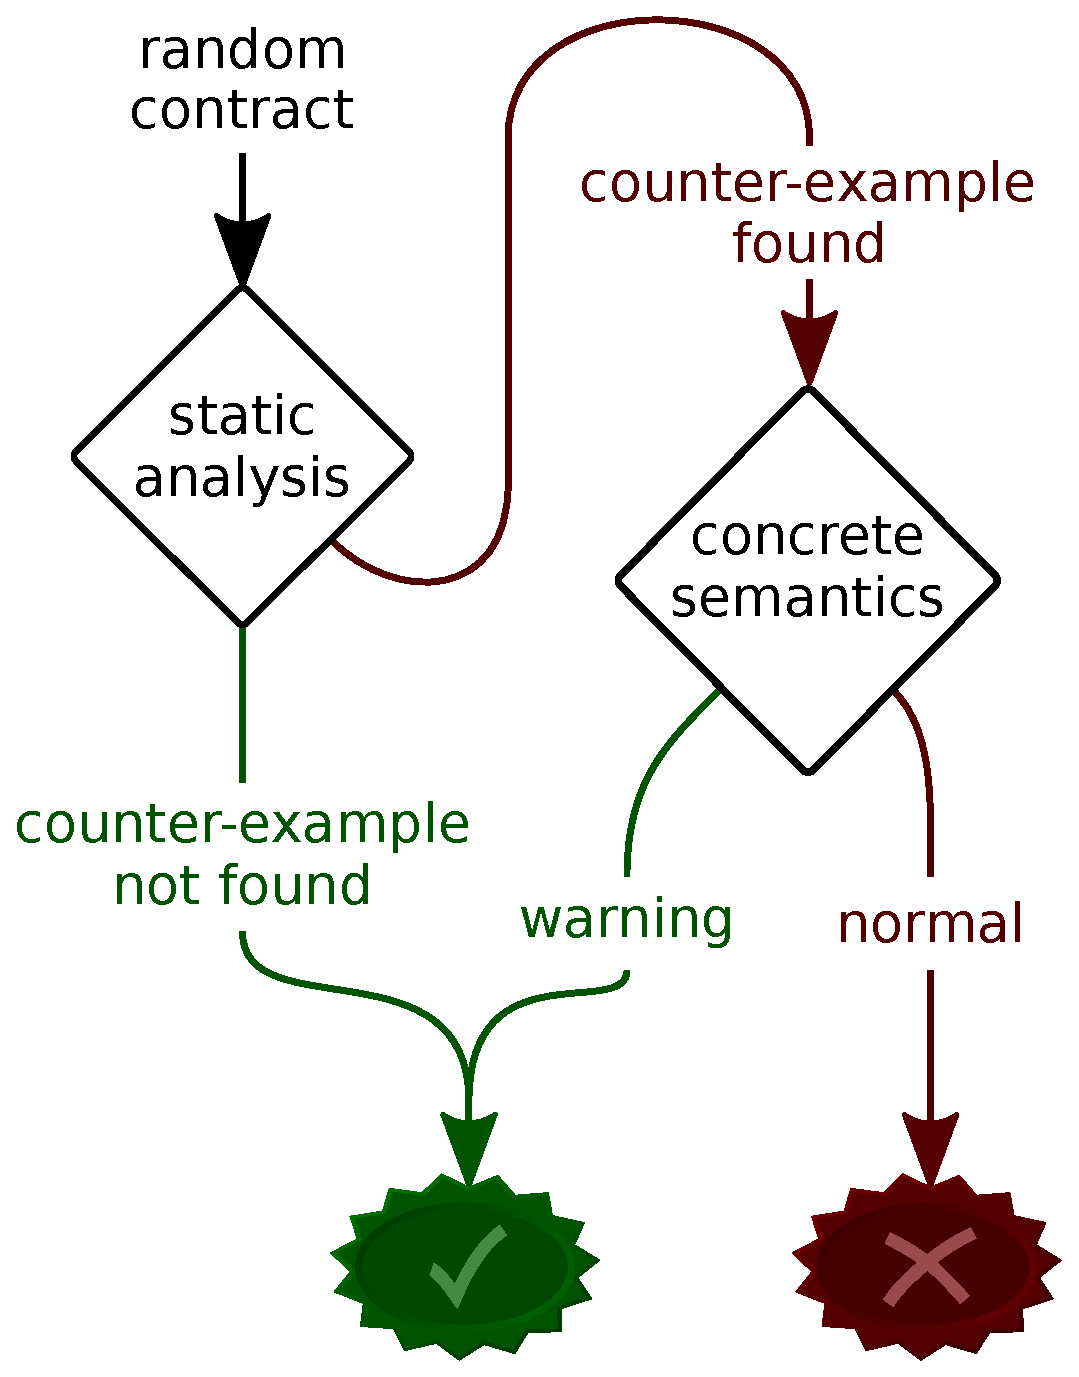
\includegraphics[width=0.5\textwidth]{figures/consistency_property}
\par\end{centering}
\caption{Property based testing for consistency\label{fig:Property-based-testing-for-consistency}}

\end{figure}


\subsection{Testing for equivalence\label{subsec:Testing-for-equivalence} }

If we have two static analysis implementations, we have another opportunity
for testing. In our case, we have one efficient implementation that
is very different from the semantics and one inefficient implementation
that is much closer to the semantics, and we can compare the results of the
two implementations. We can do this as shown in Figure~\ref{fig:Property-based-testing-for-equivalence}.
We generate random contracts using a custom QuickCheck \cite{quickcheck} generator,
we feed them to both static analysis implementations, and we compare the results.
If the results are the same then test passes, if they are different then
one of the implementations is wrong.

\begin{figure}
\begin{centering}
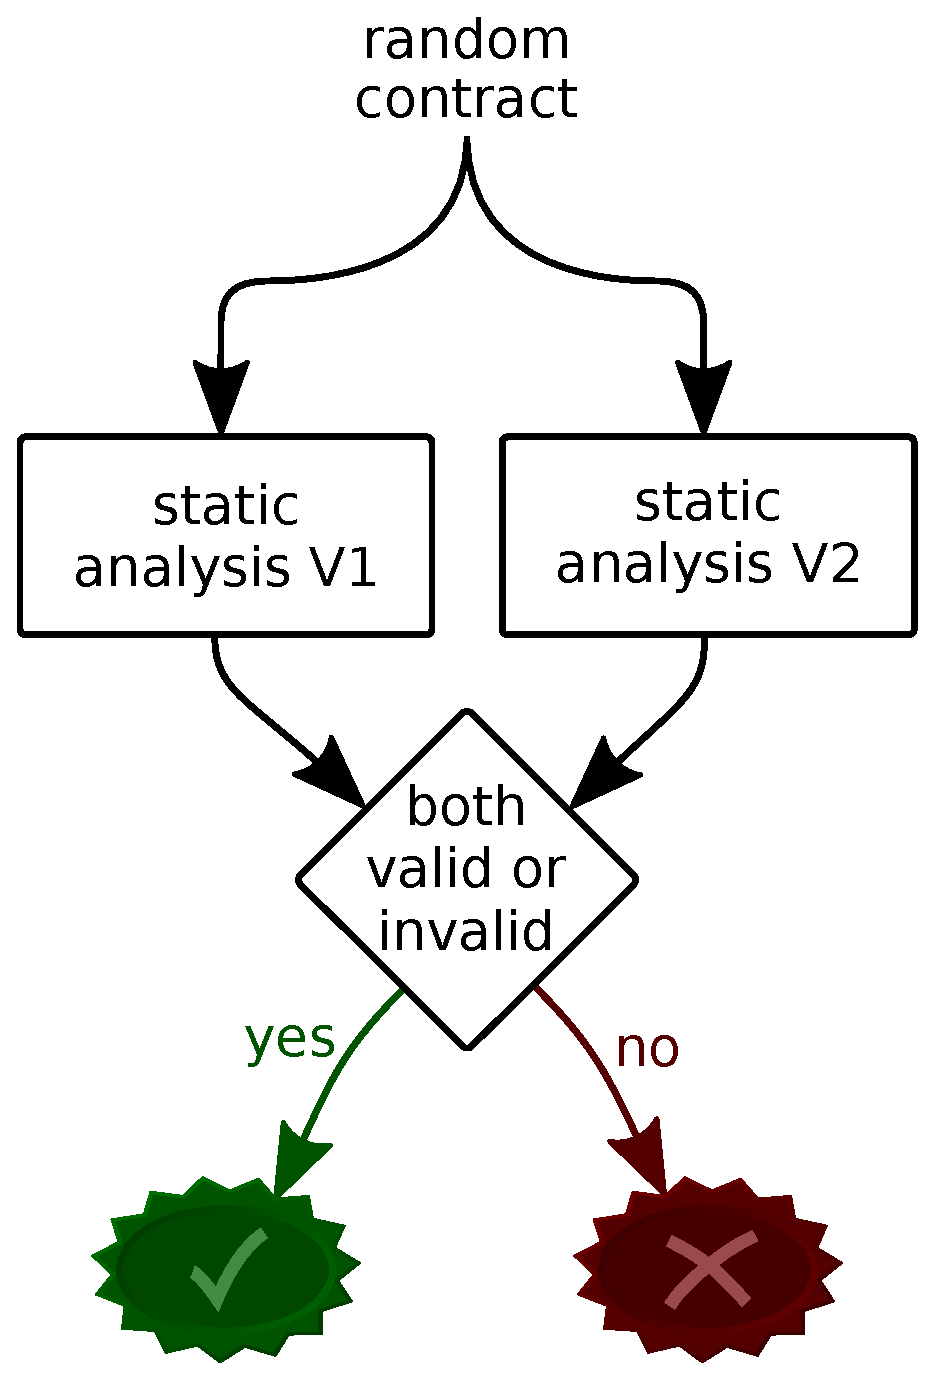
\includegraphics[width=0.45\textwidth]{figures/equivalence_property}
\par\end{centering}
\caption{Property based testing for equivalence\label{fig:Property-based-testing-for-equivalence}}
\end{figure}

This approach covers both types of errors, i.e: false positives and
false negatives (for both of the implementations), but the execution
time of the tests is bounded from below by the slower of the two implementations.
The consistency approach is thus more efficient in finding false positives.

\section{Measurements \label{sec:Measurements} }


\begin{table}[]
\centering
\scalebox{0.8}{
\begin{tabular}{l||lllll}
\multicolumn{6}{l}{\textbf{Auction contract -- \texttt{Auction.hs}}} \\ \hline \hline
\multicolumn{6}{c}{\textbf{Lightweight optimisations}} \\ \hline \hline
\textbf{Num.~participants}             & \multicolumn{1}{c|}{1}        & \multicolumn{1}{c|}{2}            & \multicolumn{1}{c|}{3}                         & \multicolumn{1}{c|}{4}                        & \multicolumn{1}{c}{5}    \\ \hline
\textbf{Execution time}                & \multicolumn{1}{c|}{0.2205s}  & \multicolumn{1}{c|}{4m 45.2015s}  & \multicolumn{1}{c|}{\color[HTML]{888888} N/A}  & \multicolumn{1}{c|}{\color[HTML]{888888} N/A} & \multicolumn{1}{c}{\color[HTML]{888888} N/A} \\ \hline
Generation overhead                    & \multicolumn{1}{c|}{76.61\%}  & \multicolumn{1}{c|}{96.40\%}      & \multicolumn{1}{c|}{\color[HTML]{888888} N/A}  & \multicolumn{1}{c|}{\color[HTML]{888888} N/A} & \multicolumn{1}{c}{\color[HTML]{888888} N/A} \\ \hline
\multicolumn{1}{r||}{× execution time} & \multicolumn{1}{c|}{0.1689s}  & \multicolumn{1}{c|}{4m 34.9342s}  & \multicolumn{1}{c|}{\color[HTML]{888888} N/A}  & \multicolumn{1}{c|}{\color[HTML]{888888} N/A} & \multicolumn{1}{c}{\color[HTML]{888888} N/A} \\ \hline
Z3 overhead                            & \multicolumn{1}{c|}{23.39\%}  & \multicolumn{1}{c|}{3.60\%}       & \multicolumn{1}{c|}{\color[HTML]{888888} N/A}  & \multicolumn{1}{c|}{\color[HTML]{888888} N/A} & \multicolumn{1}{c}{\color[HTML]{888888} N/A} \\ \hline
\multicolumn{1}{r||}{× execution time} & \multicolumn{1}{c|}{0.0516s}  & \multicolumn{1}{c|}{10.2673s}     & \multicolumn{1}{c|}{\color[HTML]{888888} N/A}  & \multicolumn{1}{c|}{\color[HTML]{888888} N/A} & \multicolumn{1}{c}{\color[HTML]{888888} N/A} \\ \hline
\textbf{RAM usage peak}                & \multicolumn{1}{c|}{44,248KB} & \multicolumn{1}{c|}{1,885,928KB}  & \multicolumn{1}{c|}{\color[HTML]{888888} N/A}  & \multicolumn{1}{c|}{\color[HTML]{888888} N/A} & \multicolumn{1}{c}{\color[HTML]{888888} N/A} \\ \hline \hline
\multicolumn{6}{c}{\textbf{Heavyweight optimisations}} \\ \hline \hline
\textbf{Num.~participants}             & \multicolumn{1}{c|}{1}          & \multicolumn{1}{c|}{2}         & \multicolumn{1}{c|}{3}         & \multicolumn{1}{c|}{4}              & \multicolumn{1}{c}{5}    \\ \hline
\textbf{Execution time}                & \multicolumn{1}{c|}{0.01198s}   & \multicolumn{1}{c|}{0.0289s}   & \multicolumn{1}{c|}{1.1138s}   & \multicolumn{1}{c|}{1h 5m 45.1377s} & \multicolumn{1}{c}{\color[HTML]{888888} N/A} \\ \hline
Generation overhead                    & \multicolumn{1}{c|}{16.27\%}    & \multicolumn{1}{c|}{29.64\%}   & \multicolumn{1}{c|}{24.09\%}   & \multicolumn{1}{c|}{80.86\%}        & \multicolumn{1}{c}{\color[HTML]{888888} N/A} \\ \hline
\multicolumn{1}{r||}{× execution time} & \multicolumn{1}{c|}{0.001949s}  & \multicolumn{1}{c|}{0.008566s} & \multicolumn{1}{c|}{0.268314s} & \multicolumn{1}{c|}{53m 10.038344s} & \multicolumn{1}{c}{\color[HTML]{888888} N/A} \\ \hline
Z3 overhead                            & \multicolumn{1}{c|}{83.73\%}    & \multicolumn{1}{c|}{70.36\%}   & \multicolumn{1}{c|}{75.91\%}   & \multicolumn{1}{c|}{19.14\%}        & \multicolumn{1}{c}{\color[HTML]{888888} N/A} \\ \hline
\multicolumn{1}{r||}{× execution time} & \multicolumn{1}{c|}{0.010031s}  & \multicolumn{1}{c|}{0.020334s} & \multicolumn{1}{c|}{0.845486s} & \multicolumn{1}{c|}{12m 35.099356s} & \multicolumn{1}{c}{\color[HTML]{888888} N/A} \\ \hline
\textbf{RAM usage peak}                & \multicolumn{1}{c|}{17,020KB}   & \multicolumn{1}{c|}{17,740KB}  & \multicolumn{1}{c|}{49,668KB}  & \multicolumn{1}{c|}{2,364,500KB}    & \multicolumn{1}{c}{\color[HTML]{888888} N/A} \\ \hline \hline
\textbf{Contract size (chars)}         & \multicolumn{1}{c|}{275}        & \multicolumn{1}{c|}{3,399}     & \multicolumn{1}{c|}{89,335}    & \multicolumn{1}{c|}{4,747,361}      & \multicolumn{1}{c}{413,784,559}
\end{tabular}
}
%\caption{Execution cost measurement of auction contract\label{table1}}
\end{table}

\begin{table}[]
\centering
\scalebox{0.8}{
\begin{tabular}{l||lllll}
\multicolumn{6}{l}{\textbf{Crowdfunding contract -- \texttt{CrowdFunding.hs}}} \\ \hline \hline
\multicolumn{6}{c}{\textbf{Lightweight optimisations}} \\ \hline \hline
\textbf{Num.~participants}             & \multicolumn{1}{c|}{1}         & \multicolumn{1}{c|}{2}            & \multicolumn{1}{c|}{3}                        & \multicolumn{1}{c|}{4}                        & \multicolumn{1}{c}{5}    \\ \hline
\textbf{Execution time}                & \multicolumn{1}{c|}{0.6298s}   & \multicolumn{1}{c|}{50m 53.4597s} & \multicolumn{1}{c|}{\color[HTML]{888888} N/A} & \multicolumn{1}{c|}{\color[HTML]{888888} N/A} & \multicolumn{1}{c}{\color[HTML]{888888} N/A} \\ \hline
Generation overhead                    & \multicolumn{1}{c|}{85.02\%}   & \multicolumn{1}{c|}{99.82\%}      & \multicolumn{1}{c|}{\color[HTML]{888888} N/A} & \multicolumn{1}{c|}{\color[HTML]{888888} N/A} & \multicolumn{1}{c}{\color[HTML]{888888} N/A} \\ \hline
\multicolumn{1}{r||}{× execution time} & \multicolumn{1}{c|}{0.5356s}   & \multicolumn{1}{c|}{50m 47.9635s} & \multicolumn{1}{c|}{\color[HTML]{888888} N/A} & \multicolumn{1}{c|}{\color[HTML]{888888} N/A} & \multicolumn{1}{c}{\color[HTML]{888888} N/A} \\ \hline
Z3 overhead                            & \multicolumn{1}{c|}{14.98\%}   & \multicolumn{1}{c|}{0.18\%}       & \multicolumn{1}{c|}{\color[HTML]{888888} N/A} & \multicolumn{1}{c|}{\color[HTML]{888888} N/A} & \multicolumn{1}{c}{\color[HTML]{888888} N/A} \\ \hline
\multicolumn{1}{r||}{× execution time} & \multicolumn{1}{c|}{0.0943s}   & \multicolumn{1}{c|}{5.4962s}      & \multicolumn{1}{c|}{\color[HTML]{888888} N/A} & \multicolumn{1}{c|}{\color[HTML]{888888} N/A} & \multicolumn{1}{c}{\color[HTML]{888888} N/A} \\ \hline
\textbf{RAM usage peak}                & \multicolumn{1}{c|}{111,980KB} & \multicolumn{1}{c|}{5,641,056KB}  & \multicolumn{1}{c|}{\color[HTML]{888888} N/A} & \multicolumn{1}{c|}{\color[HTML]{888888} N/A} & \multicolumn{1}{c}{\color[HTML]{888888} N/A} \\ \hline \hline
\multicolumn{6}{c}{\textbf{Heavyweight optimisations}} \\ \hline \hline
\textbf{Num.~participants}             & \multicolumn{1}{c|}{1}        & \multicolumn{1}{c|}{2}        & \multicolumn{1}{c|}{3}        & \multicolumn{1}{c|}{4}            & \multicolumn{1}{c}{5}    \\ \hline
\textbf{Execution time}                & \multicolumn{1}{c|}{0.0125s}  & \multicolumn{1}{c|}{0.041s}   & \multicolumn{1}{c|}{1.0515s}  & \multicolumn{1}{c|}{32m 15.4478s} & \multicolumn{1}{c}{\color[HTML]{888888} N/A} \\ \hline
Generation overhead                    & \multicolumn{1}{c|}{16.68\%}  & \multicolumn{1}{c|}{25.36\%}  & \multicolumn{1}{c|}{37.23\%}  & \multicolumn{1}{c|}{69.83\%}      & \multicolumn{1}{c}{\color[HTML]{888888} N/A} \\ \hline
\multicolumn{1}{r||}{× execution time} & \multicolumn{1}{c|}{0.0021s}  & \multicolumn{1}{c|}{0.0104s}  & \multicolumn{1}{c|}{0.3915s}  & \multicolumn{1}{c|}{22m 31.5232s} & \multicolumn{1}{c}{\color[HTML]{888888} N/A} \\ \hline
Z3 overhead                            & \multicolumn{1}{c|}{83.32\%}  & \multicolumn{1}{c|}{74.64\%}  & \multicolumn{1}{c|}{62.77\%}  & \multicolumn{1}{c|}{30.17\%}      & \multicolumn{1}{c}{\color[HTML]{888888} N/A} \\ \hline
\multicolumn{1}{r||}{× execution time} & \multicolumn{1}{c|}{0.0104s}  & \multicolumn{1}{c|}{0.0306s}  & \multicolumn{1}{c|}{0.6600s}  & \multicolumn{1}{c|}{9m 43.9246s}  & \multicolumn{1}{c}{\color[HTML]{888888} N/A} \\ \hline
\textbf{RAM usage peak}                & \multicolumn{1}{c|}{17,016KB} & \multicolumn{1}{c|}{18,768KB} & \multicolumn{1}{c|}{62,108KB} & \multicolumn{1}{c|}{3,715,020KB}  & \multicolumn{1}{c}{\color[HTML]{888888} N/A} \\ \hline \hline
\textbf{Contract size (chars)}         & \multicolumn{1}{c|}{857}      & \multicolumn{1}{c|}{12,704}   & \multicolumn{1}{c|}{364,824}  & \multicolumn{1}{c|}{19,462,278}   & \multicolumn{1}{c}{1,690,574,798}
\end{tabular}
}
%\caption{Execution cost measurement of crowdfunding contract\label{table2}}
\end{table}

\begin{table}[]
\centering
\scalebox{0.8}{
\begin{tabular}{l||lllll}
\multicolumn{6}{l}{\textbf{Rent contract -- \texttt{Rent.hs}}} \\ \hline \hline
\multicolumn{6}{c}{\textbf{Lightweight optimisations}} \\ \hline \hline
\textbf{Num.~months}                   & \multicolumn{1}{c|}{1}        & \multicolumn{1}{c|}{2}         & \multicolumn{1}{c|}{3}           & \multicolumn{1}{c|}{4}               & \multicolumn{1}{c}{5}    \\ \hline
\textbf{Execution time}                & \multicolumn{1}{c|}{0.2850s}  & \multicolumn{1}{c|}{3.0303s}   & \multicolumn{1}{c|}{2m 53.2458s} & \multicolumn{1}{c|}{3h 22m 13.0122s} & \multicolumn{1}{c}{\color[HTML]{888888} N/A} \\ \hline
Generation overhead                    & \multicolumn{1}{c|}{77.55\%}  & \multicolumn{1}{c|}{91.25\%}   & \multicolumn{1}{c|}{99.18\%}     & \multicolumn{1}{c|}{99.94\%}         & \multicolumn{1}{c}{\color[HTML]{888888} N/A} \\ \hline
\multicolumn{1}{r||}{× execution time} & \multicolumn{1}{c|}{0.2210s}  & \multicolumn{1}{c|}{2.7651s}   & \multicolumn{1}{c|}{2m 51.8252s} & \multicolumn{1}{c|}{3h 22m 5.7324s}  & \multicolumn{1}{c}{\color[HTML]{888888} N/A} \\ \hline
Z3 overhead                            & \multicolumn{1}{c|}{22.45\%}  & \multicolumn{1}{c|}{8.75\%}    & \multicolumn{1}{c|}{0.82\%}      & \multicolumn{1}{c|}{0.06\%}          & \multicolumn{1}{c}{\color[HTML]{888888} N/A} \\ \hline
\multicolumn{1}{r||}{× execution time} & \multicolumn{1}{c|}{0.0640s}  & \multicolumn{1}{c|}{0.2652s}   & \multicolumn{1}{c|}{1.4206s}  & \multicolumn{1}{c|}{7.2798s}         & \multicolumn{1}{c}{\color[HTML]{888888} N/A} \\ \hline
\textbf{RAM usage peak}                & \multicolumn{1}{c|}{42,052KB} & \multicolumn{1}{c|}{221,960KB} & \multicolumn{1}{c|}{1,237,092KB} & \multicolumn{1}{c|}{9,160,616KB}     & \multicolumn{1}{c}{\color[HTML]{888888} N/A} \\ \hline \hline
\multicolumn{6}{c}{\textbf{Heavyweight optimisations}} \\ \hline \hline
\textbf{Num.~months}                   & \multicolumn{1}{c|}{1}        & \multicolumn{1}{c|}{2}        & \multicolumn{1}{c|}{3}        & \multicolumn{1}{c|}{4}        & \multicolumn{1}{c}{5}    \\ \hline
\textbf{Execution time}                & \multicolumn{1}{c|}{0.0114s}  & \multicolumn{1}{c|}{0.0111s}  & \multicolumn{1}{c|}{0.01132s} & \multicolumn{1}{c|}{0.01124s} & \multicolumn{1}{c}{0.01255s} \\ \hline
Generation overhead                    & \multicolumn{1}{c|}{11.55\%}  & \multicolumn{1}{c|}{11.95\%}  & \multicolumn{1}{c|}{13.65\%}  & \multicolumn{1}{c|}{13.69\%}  & \multicolumn{1}{c}{21.00\%} \\ \hline
\multicolumn{1}{r||}{× execution time} & \multicolumn{1}{c|}{0.0013s}  & \multicolumn{1}{c|}{0.0013s}  & \multicolumn{1}{c|}{0.0015s}  & \multicolumn{1}{c|}{0.0015s}  & \multicolumn{1}{c}{0.0026s} \\ \hline
Z3 overhead                            & \multicolumn{1}{c|}{88.45\%}  & \multicolumn{1}{c|}{88.05\%}  & \multicolumn{1}{c|}{86.35\%}  & \multicolumn{1}{c|}{86.31\%}  & \multicolumn{1}{c}{79.00\%} \\ \hline
\multicolumn{1}{r||}{× execution time} & \multicolumn{1}{c|}{0.0101s}  & \multicolumn{1}{c|}{0.0098s}  & \multicolumn{1}{c|}{0.0098s}  & \multicolumn{1}{c|}{0.0097s}  & \multicolumn{1}{c}{0.0099s} \\ \hline
\textbf{RAM usage peak}                & \multicolumn{1}{c|}{15,536KB} & \multicolumn{1}{c|}{15,364KB} & \multicolumn{1}{c|}{15,400KB} & \multicolumn{1}{c|}{15,364KB} & \multicolumn{1}{c}{15,540KB} \\ \hline \hline
\textbf{Contract size (chars)}         & \multicolumn{1}{c|}{339}      & \multicolumn{1}{c|}{595}      & \multicolumn{1}{c|}{852}      & \multicolumn{1}{c|}{1,109}    & \multicolumn{1}{c}{1,366}
\end{tabular}
}
%\caption{Execution cost measurement of crowdfunding contract\label{table3}}
\end{table}

\begin{table}[]
\centering
\scalebox{0.8}{
\begin{tabular}{l||lllll}
\multicolumn{6}{l}{\textbf{Coupon bond contract - ACTUS.hs}} \\ \hline \hline
\multicolumn{6}{c}{\textbf{Lightweight optimisations}} \\ \hline \hline
\textbf{Num.~months}                   & \multicolumn{1}{c|}{2}        & \multicolumn{1}{c|}{3}         & \multicolumn{1}{c|}{4}           & \multicolumn{1}{c|}{5}            & \multicolumn{1}{c}{6}    \\ \hline
\textbf{Execution time}                & \multicolumn{1}{c|}{0.8293s}  & \multicolumn{1}{c|}{5.8887s}   & \multicolumn{1}{c|}{1m 35.3930s} & \multicolumn{1}{c|}{26m 36.4585s} & \multicolumn{1}{c}{9h 50m 22.3418s} \\ \hline
Generation overhead                    & \multicolumn{1}{c|}{76.57\%}  & \multicolumn{1}{c|}{74.91\%}   & \multicolumn{1}{c|}{89.29\%}     & \multicolumn{1}{c|}{72.34\%}      & \multicolumn{1}{c}{76.66\%} \\ \hline
\multicolumn{1}{r||}{× execution time} & \multicolumn{1}{c|}{0.6350s}  & \multicolumn{1}{c|}{4.4112s}   & \multicolumn{1}{c|}{1m 25.1764s} & \multicolumn{1}{c|}{19m 14.8781s} & \multicolumn{1}{c}{7h 32m 34.7672s} \\ \hline
Z3 overhead                            & \multicolumn{1}{c|}{23.43\%}  & \multicolumn{1}{c|}{25.09\%}   & \multicolumn{1}{c|}{10.71\%}     & \multicolumn{1}{c|}{27.66\%}      & \multicolumn{1}{c}{23.34\%} \\ \hline
\multicolumn{1}{r||}{× execution time} & \multicolumn{1}{c|}{0.1943s}  & \multicolumn{1}{c|}{1.4775s}   & \multicolumn{1}{c|}{10.2166s}    & \multicolumn{1}{c|}{7m 21.5804s}  & \multicolumn{1}{c}{2h 17m 47.5746s} \\ \hline
\textbf{RAM usage peak}                & \multicolumn{1}{c|}{74,180KB} & \multicolumn{1}{c|}{209,724KB} & \multicolumn{1}{c|}{940,924KB}   & \multicolumn{1}{c|}{3,283,384KB}  & \multicolumn{1}{c}{13,483,908KB} \\ \hline \hline
\multicolumn{6}{c}{\textbf{Heavyweight optimisations}} \\ \hline \hline
\textbf{Num.~months}                   & \multicolumn{1}{c|}{2}        & \multicolumn{1}{c|}{3}        & \multicolumn{1}{c|}{4}        & \multicolumn{1}{c|}{5}        & \multicolumn{1}{c}{6}    \\ \hline
\textbf{Execution time}                & \multicolumn{1}{c|}{0.0092s}  & \multicolumn{1}{c|}{0.0095s}  & \multicolumn{1}{c|}{0.0097s}  & \multicolumn{1}{c|}{0.0102s}  & \multicolumn{1}{c}{0.0105s} \\ \hline
Generation overhead                    & \multicolumn{1}{c|}{14.51\%}  & \multicolumn{1}{c|}{15.50\%}  & \multicolumn{1}{c|}{15.51\%}  & \multicolumn{1}{c|}{19.71\%}  & \multicolumn{1}{c}{19.69\%} \\ \hline
\multicolumn{1}{r||}{× execution time} & \multicolumn{1}{c|}{0.0013s}  & \multicolumn{1}{c|}{0.0015s}  & \multicolumn{1}{c|}{0.0015s}  & \multicolumn{1}{c|}{0.0020s}  & \multicolumn{1}{c}{0.0021s} \\ \hline
Z3 overhead                            & \multicolumn{1}{c|}{85.49\%}  & \multicolumn{1}{c|}{84.50\%}  & \multicolumn{1}{c|}{84.49\%}  & \multicolumn{1}{c|}{80.29\%}  & \multicolumn{1}{c}{80.31\%} \\ \hline
\multicolumn{1}{r||}{× execution time} & \multicolumn{1}{c|}{0.0079s}  & \multicolumn{1}{c|}{0.0080s}  & \multicolumn{1}{c|}{0.0082s}  & \multicolumn{1}{c|}{0.0082s}  & \multicolumn{1}{c}{0.0085s} \\ \hline
\textbf{RAM usage peak}                & \multicolumn{1}{c|}{15,636KB} & \multicolumn{1}{c|}{15,816KB} & \multicolumn{1}{c|}{15,788KB} & \multicolumn{1}{c|}{15,780KB} & \multicolumn{1}{c}{15,760KB} \\ \hline \hline
\textbf{Contract size (chars)}         & \multicolumn{1}{c|}{479}      & \multicolumn{1}{c|}{635}      & \multicolumn{1}{c|}{791}      & \multicolumn{1}{c|}{947}      & \multicolumn{1}{c}{1,103}
\end{tabular}
}
%\caption{Execution cost measurement of coupon contract\label{table4}}
\vspace*{-0.6cm}
\end{table}

In our experiments, the heavyweight optimisations considerably reduced
the requirements of both processing time and memory for Marlowe's static
analysis. %In Tables~\ref{table1},~\ref{table2},~\ref{table3},~and~\ref{table4},
We present below the results of measuring the performance of static analysis on
four example  contracts,
before\footnote{\url{https://github.com/input-output-hk/marlowe/blob/master/src/Language/Marlowe/Analysis/FSSemantics.hs} [last visited 19-05-2020]}
and after\footnote{\url{https://github.com/input-output-hk/marlowe/blob/master/src/Language/Marlowe/Analysis/FSSemanticsFastVerbose.hs} [last visited 19-05-2020]}
the heavyweight optimisations.

\noindent
Unfortunately, at the time of writing, we do not have a completely unoptimised
version of the static analysis that we can use to compare, because the semantics
of Marlowe have changed since we implemented that version. However, our impression
from manual testing is that the impact of lightweight optimisations was much more modest than the impact of heavyweight optimisations.

Using the \texttt{perf} tool \cite{perf}, we have measured the execution
time\footnote{The experiments were run on a laptop computer with a
i9-9900K (3.6GHz) processor and two modules of 16GB of SODIMM DDR4 RAM at 2400MHz.}
and the overhead of both the generation of the constraints and their solution
by Z3 \cite{de2008z3}. And we have measured the peak RAM usage of the whole
process by using GNU's \texttt{time} tool \cite{keppel1998gnu}.

In all the contracts, the implementation that has the heavyweight optimisations
performs much better and scales further. In the case of the \textit{auction}
and \textit{crowdfunding} contracts, whose size grows exponentially, both
approaches quickly overwhelm the resources available in the execution environment.
On the other hand, in the case of \textit{rent} and \textit{coupon bond} contracts,
which grow linearly, by using the lightweight version, the problem becomes 
intractable much faster than with the heavyweight version.

Another conclusion that can be derived from the experiments is that, in the
version with lightweight optimisations, most of the processing time seems to be
spent generating of the constraints, and solving is done relatively
quickly by Z3; while the opposite happens for the version with heavyweight
optimisations.

These results suggest that the SBV library is able to generate constraints in a way
that they are handled efficiently by Z3, but the process itself can be costly
if we are not careful. Nevertheless, the overall execution time required by Z3
is also lower in the case of the version with heavyweight optimisations and it
grows more slowly, which suggests the optimisations described in this paper
affect both stages of the process to some extent.

\section{Related work}

Work in \cite{mokhov2019formal} documents a similar effort to ensure
correctness of implementations by using Haskell and SBV library; the
authors also discuss performance of the analysis and apply this approach
to non-functional requirements.

The idea of using constraint solvers for finding bugs is not new,
and there has been a number of initiatives that have explored its
application to the verification of assertions in programs written
using general purpose programming languages \cite{gulwani2008program,jackson2000finding};
as well as for the compliance with usage protocols
\cite{ball2001automatically,xie2005saturn}.

\cite{keshishzadeh2013early} also applies constraint solvers for
detecting problems in the usage of DSLs. The authors observe that
SMT solvers have limited support for non-linear constraints such as
exponentiation. This problem does not affect the current design of
Marlowe because it does not support multiplication by arbitrary variables,
and because all inputs are integer and bounded finitely.

\section{Future work}

In the future, we would like to extend static analysis to cover other
potential problems in Marlowe contracts and to aid their development.
We can envisage that we can use static analysis to locate unreachable
subcontracts, to allow developers to provide custom assertions and
check their satisfiability, and even to allow users to inspect the
possible maximum and minimum values that particular expressions can
reach. 

\section{Conclusion}

In this paper, we have summarized the lessons learned from our work
on optimising the static analysis for Marlowe contracts. We have found
that there are two clear approaches to static analysis using SMT,
both have advantages and disadvantages. One is less error prone and
straightforward, but inefficient and hard to test; the other approach
is much more efficient, versatile, and testable, but more error prone.

We have also seen that many specific properties and restrictions characteristic
of the target DSL can be utilized both as optimisation opportunities
and, in our case, for completeness of the analysis. Symbolic execution
of, for example, a turing complete language, would be intractable,
and would require us to manually set a bound; but this is not in the
case for Marlowe.

In the end, we have illustrated how to counteract the main disadvantage
of the later approach, its propensity to errors, by using property
based testing. This way we have obtained a static analysis implementation
that is efficient, versatile, testable, and reliable.

On the other hand, for the static analysis of Marlowe contracts, we
found out that when running statistics on the equivalence testing
property, most of the bugs were false negatives in the straightforward
implementation, and the optimised implementation seems to be more
reliable thanks to the consistency tests that we run beforehand.

Another advantage of the optimised implementation is that, because
it relies on fewer and simpler features, it is compatible with more
SMT solvers which, in turn, means that it is less reliant on the
correctness of a single SMT solver. If an SMT solver fails to give
an answer, we can try a different one; if we want to ensure that a
contract is valid, we can test it with several SMT solvers and ensure
all of them agree. 

\bibliographystyle{splncs04}
\bibliography{paper}

\end{document}
